To further demonstrate how the eigenspace overlap metric can be used to better understand the performance of compressed embeddings, in this section we show that we can upper bound the eigenspace overlap for uniformly quantized embeddings.
Given the above theoretical and empirical connections between eigenspace overlap and generalization performance, these bounds help explain why the uniformly quantized embeddings perform so well.
To prove these bounds, we leverage the classic Davis-Kahan $\sin(\Theta)$ theorem from matrix perturbation analysis \citep{sintheta70}.
Because we know exactly what the noise structure of the uniform quantization method is, we can use this knowledge to bound how much the eigenspace of the compressed embeddings can differ from the uncompressed embeddings.

We now present the result (see Appendix~\ref{app:theory} for proof):
\begin{theorem}
	Let $X \in \RR^{n\times d}$ be a bounded embedding matrix with $X_{ij} \in [-\frac{1}{\sqrt{d}},\frac{1}{\sqrt{d}}]$ with smallest singular value $\sigma_{\min} = a \sqrt{n/d}$, for $a \in [0,1]$.\footnote{The maximum possible value of $\sigma_{\min}$ is $\sqrt{n/d}$, which occurs when $\|X\|_F^2 = n$ and $\sigma_{\min} = \sigma_{\max}$.}
	Then the eigenspace overlap of the corresponding $b$-bit uniformly quantized embedding matrix can be lower bounded as follows:
	\begin{eqnarray*}
		%\eigover(X,\tX) &\geq& 1 - \frac{16n}{d(2^b-1)^2} \Bigg( \frac{\sigma_{\max} + \frac{\sqrt{n}}{2^b-1} }{\sigma_{\min}^2} \Bigg)^2
		\expect{}{1-\eigover(X,\tX)} &\leq& \frac{20 \delta_b^2}{a^4}
	\end{eqnarray*}
\label{thm1}
\end{theorem}

This theorem directly results in the following corollary:
%\begin{corollary}
%If $b \geq \log_2\bigg(\frac{8n}{\sigma_{\min}^2 \sqrt{\rho \, d} }} + 1\bigg)$, then the $b$-bit uniformly quantized embedding matrix $\tX$ satisfies $\eigover(X,\tX) \geq 1-\rho$.
%\end{corollary}
\begin{corollary}
	$$\expect{}{1-\eigover(X,\tX)} \leq \eps \;\;\text{if}\;\; b \geq \log_2\bigg(\frac{\sqrt{20}}{a^2\sqrt{\eps}}+1\bigg).$$
\end{corollary}
The corollary shows that one can attain an expected eigenspace overlap arbitrarily close to $1$ if a sufficient number of bits $b$ are used.

\paragraph{Empirical Validation of Theory}
We now validate the above theory by showing how the eigenspace overlap grows as the precision of the uniformly quantized embeddings is increased.
For this experiment, we generate a random matrix $X \in \RR^{10^5 \times 300}$, with each entry drawn uniformly at random in the interval $[-\frac{1}{\sqrt{300}}, \frac{1}{\sqrt{300}}]$.
We then measure the eigenspace overlap of quantized versions of $X$, for precisions $b \in \{1,2,4,8,16,32\}$.
As we can see in Figure~\ref{fig:micro_eigoverlap_vs_prec}, the eigenspace overlap grows quite quickly as the precision grows, attaining a value of approximately $0.82$ at $b=2$, and $0.99$ at $b=4$.
This helps explain the strong empirical performance of the uniformly quantized embeddings which we observed at low precisions on the real word embedding experiments (Figure~\ref{fig:perf_comp}).

%\todo{Add section on clippings effect on the eigenspace overlap?}

\begin{figure}
	\begin{tabular}{c}
		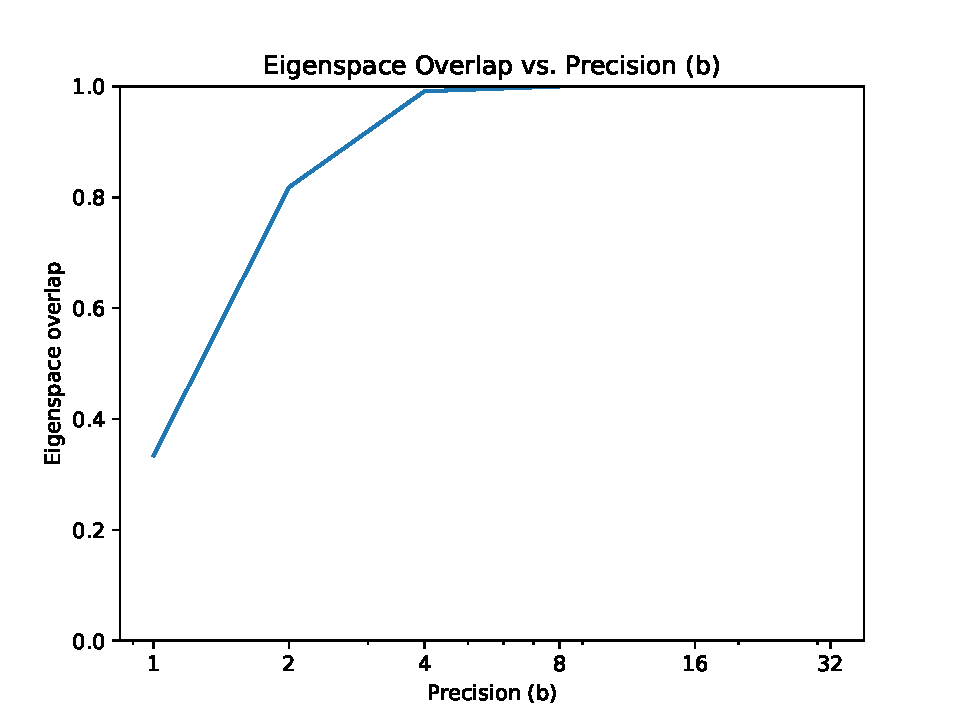
\includegraphics[width=\linewidth]{figures/micro_eig_overlap_vs_precision.pdf} 
\end{tabular}
\caption{Empirical Validation of Theorem~\ref{thm1}. We measure the eigenspace overlap of uniformly quantized embeddings with the uncompressed embedding for various precisions ($b\in\{1,2,4,8,16,32\}$), and observe the eigenspace overlap grows quickly as the precision grows.  For the uncompressed embedding, we generate a random matrix $X \in \RR^{10^5 \times 300}$, with each entry drawn uniformly at random in $[-\frac{1}{\sqrt{300}}, \frac{1}{\sqrt{300}}]$.}
\label{fig:micro_eigoverlap_vs_prec}
\end{figure}

%\subsection{Theory validation}
%	\begin{itemize}
%		\item Impact of quantization on overlap 
%			\begin{itemize}
% 				\item Exp 1: overlap vs precision for different dimensionality. Expectation: overlap increases with higher precision.
%				\item Exp2: overlap vs dimensionality for different precision. Expectation: overlap increases with dimensionality. This explains that under fix memory budget, using lower bits quantization can be beneficial
%			\end{itemize}
%		\item The impact of clipping on eigen-subspace overlap
%			\begin{itemize}
%				\item Simulation based experiments on subspace overlap as a function of different clipping threshold and precision. 
%				\item The way we introduce this in: in our main theorem, we assume the dynamic range is $O(1/\sqrt{d})$ as a consequence of the automatic clipping. We want to show here this is the case in practice and then discuss the specific way clipping influence eigenspace overlap.
%			\end{itemize}
%		\item Loop-back discussion on the large scale empirical experiments in Section~\ref{subsec:hard_explain}
%	\end{itemize}
